\documentclass[pdftex]{article}
\usepackage{float}
\usepackage{graphicx}
\usepackage{hyperref}
\usepackage{amsmath}

\DeclareMathOperator*{\argmax}{argmax}

\newcommand{\mC}[1]{$^\textrm{m#1}$C}
\newcommand{\mA}{$^\textrm{m6}$A}

\oddsidemargin  0.0in \evensidemargin 0.0in
\textwidth      6in


\begin{document}

\title{\begin{center}
\includegraphics[width=2in]{logo.jpg}\end{center}\vspace{0.5cm}
Detection and Identification of Base Modifications with Single Molecule Real-Time Sequencing Data}
\author{Patrick Marks, Onureena Banerjee, David Alexander}
\maketitle


% Will say the section an page
\pagestyle{headings}

\section{Introduction}
Single Molecule Real-Time (SMRT\textsuperscript{\textregistered}) DNA sequencing\cite{eid2009real} data contains information about DNA base modifications imprinted in the kinetics of the polymerization reaction\cite{flusberg2010direct}.  This data enables single-base resolution detection of \mA, \mC{4}, and \mC{5}\cite{clark2012characterization}. We discuss the statistical approaches to the detection and identification of DNA modifications from SMRT sequencing data.  Our implementation is available at \url{http://github.com/PacificBiosciences/kineticsTools}.


\section{Preparation of IPD data}
\label{sec:prep}

This analysis assumes that we are interested in locus-specific DNA modifications - that is, samples where the same modification is present at a given locus, in some fraction of the sample molecules.  

We compute a vector of IPDs that map confidently to a given genomic location. We use the alignment tool BLASR \cite{blasr} to generate alignments between reads and a reference template.   BLASR maps each read to the reference sequence. BLASR generates a Mapping QV representing the confidence that the read maps uniquely to the selected genomic interval.  Reads falling within repeats will have a low Mapping QV and are removed from the analysis to prevent incorrect modification calls inside repeats due to mismapped reads.

Sequencing errors in SMRT sequence data are predominately indels, which causes some ambiguity in the local placement of IPDs to genomic positions.  To avoid most of these errors we only use IPDs if the SMRT sequence matches exactly for $k$ bases around observed base. Currently we use $k=1$.

These filtering steps yield a vector of IPDs confidently assigned to each genomic position.

The distribution of IPDs observed at a genomic location is roughly exponential, with a long tail caused by polymerase pausing inherent to SMRT sequencing. Information about base modifications is contained in the main distribution, while the contaminating pauses just contribute noise.  We employ a simple capping procedure to reduce the influence of these outliers: 
$I_i^{(l)} = \min(R_i^{(l)}, Q_{99})$ where $I_i^{(l)}$ is the $i$th capped IPD at genomic location $l$, $R_i^{(l)}$ is the $i$th raw IPD and $Q_{99}$ is the $99$th percentile IPD over all IPD observations.

We summarize the capped IPDs at each positions with a sample mean and standard deviation of the mean:
\begin{eqnarray} 
\mu_l & = & \frac{1}{n_l} \sum_i R_i^{(l)} \\
\sigma_l^2 & = & \frac{1}{n_l} \sqrt{\sum_i (R_i^{(l)} - m_l)^2 }
\end{eqnarray}


\section{Control IPDs}

Modification detection proceeds by comparing the observed mean IPD $m_l$ with the expected mean IPD for unmodified DNA at that location. In case-control mode we sequence a sample of DNA from the same organism that has been \emph{whole genome amplified} (WGA) to preserve the DNA sequence while removing all base modifications. In this mode of operation we summarize the IPDs observed in the control sample in the same way as the case sample, then proceed to the modification detection step. If a control sample is used we compute $\mu_l^{(c)}$ and $\sigma_l^{(c)}$ for each position on the control sample data as in Section \ref{sec:prep}.

\subsection{\emph{in-silico} Control}
An alternative to the \emph{case-control} paradigm is to construct an \emph{in-silico} model to predict the mean IPD  unmodified DNA given the local sequence context. We use the Gradient Boosting Machines \cite{gradientboost} to construct a function $Q(\mathbf{c})$ that returns an estimate of the mean IPD given a DNA context $\mathbf{c} = \{c_{-8}, c_{-7}, ... ,c_0, c_1, .., c_3\}$ where $c_i \in \{A, C, G, T\}$ encodes the DNA sequence surrounding $c_0$. The IPD prediction $Q(\mathbf{c})$ corresponds to the IPD of base $c_0$. Initially we generated models spanning $-15$ to $+15$ base pairs to determine the appropriate size of the context vector. Figure \ref{fig:position-influence} shows the GBM variable influence measure relative to the cognate base. We chose a context window of $-8$ to $3$ by cutting off the window when the influence becomes small.  The extent of the window agrees with the set of bases interacting with the polymerase in crystal structures.  Each base $c_i$ in the context vector becomes a feature available to GBM learning machinery. We chose GBM because it naturally handles categorical feature variables, and it automatically discovers complicated variable interactions. We a shrinkage (or learning rate) of $\lambda=0.15$. We fit $T=60000$ trees in our ensemble, each with a maximum interaction depth of $K=12$  We used the \textsf{gbm} package\cite{gbm} from R for initial experiments, and a custom port of the code for production training.  The \emph{in-silico} IPD model $Q(\mathbf{c})$ will have some bias compared to the true mean at some genomic location due to noise in the training dataset that was not generalized out in the training procedure, in or due to the residual influence of sequence outside of the context window. 

\begin{eqnarray}
\mu_l^{(c)} & = & Q(\mathbf{Ctx}(l)) \\
\sigma_l^{(c)} & = & f(\mu_l^{(c)})
\end{eqnarray}

\begin{figure}
\begin{center}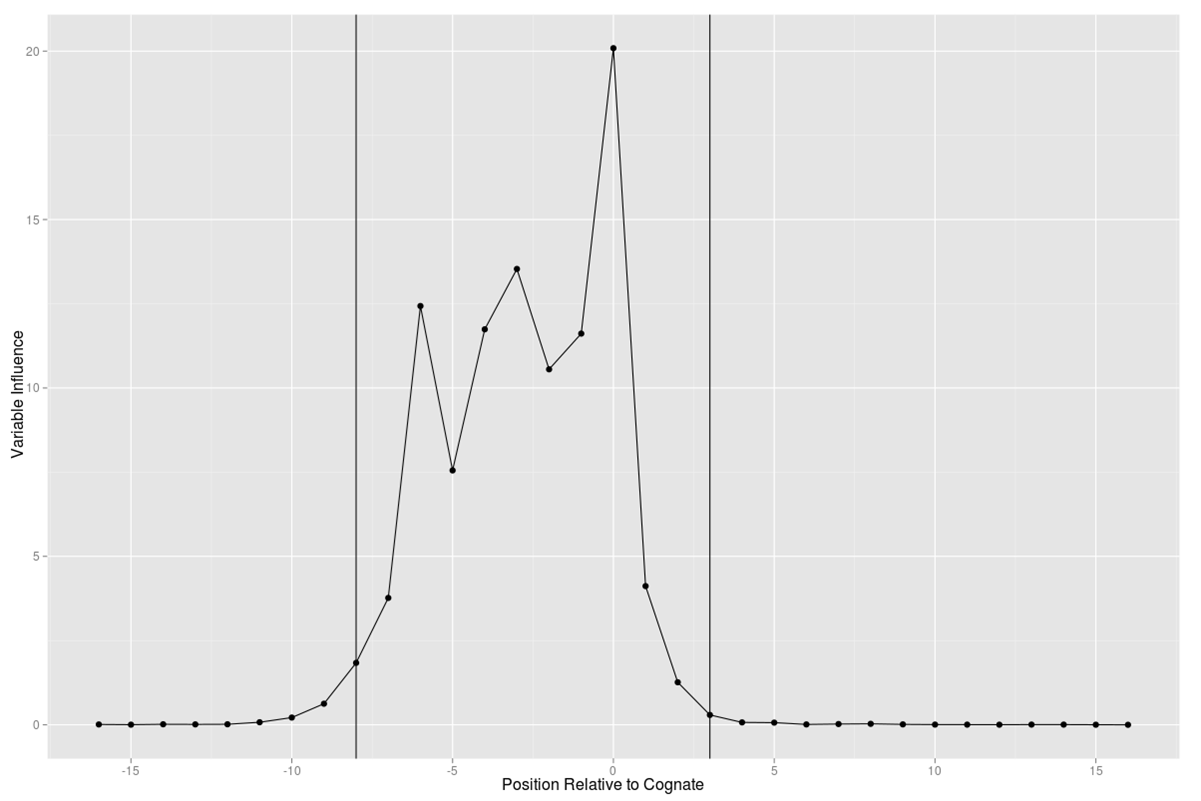
\includegraphics[width=5in]{position-influence.png}\end{center}
\caption{ Influence of Base in Context Window }
\label{fig:position-influence}
\end{figure}


\section{Modification Detection}
We pose the modification detection problem as the detection of genome locations whose mean IPD differs significantly from the control mean. We use a Welch's $t$-test to test for differences in the means between the case sample and the control, derived from either a control sample or the \emph{in-silico} model above.

The $t$-statistic is defined as:
\begin{eqnarray}
s_l & = & = \sqrt{ \sigma_l^2 + \sigma_l^{(c)2}} \\
T_l & = &\frac{\mu_l - \mu_l^{(c)}}{s_l} 
\end{eqnarray}

and we compute the p-value of $T_l$ under the $t$-distribution, and report a Phred-transformed QV as well:
\begin{eqnarray}
p & = & \Pr(t > T_l) \\
\mathrm{QV} & = & -10 \log_{10} p
\end{eqnarray}


\section{ Modification Identification } 

\subsection { Positive Control Model }
We extend the \emph{in-silico} model from an alphabet over DNA bases $c_i \in \{A,C,G,T\}$ to an alphabet that includes the \emph{modified} bases we aim to identify: $c_i \in \{A,C,G,T, ^\textrm{m6}A, ^\textrm{m5}C, ^\textrm{m4}C \}$. To train this model we require labeled examples of the modified bases in a reasonable diversity of background contexts.  Base modifications appearing in bacterial restriction-modification systems provide an excellent source of training data that is fairly straightforward to label. A typical bacteria will express several (generally between 2 and 7, going as high as 20) methyltranserases that specifically methylate a particular sequence context in the host genome. The expression of the methyltransferase is generally paired with the expression of a restriction enzyme whose recognition site matches that of the methyltransferase. These \emph{active} RM systems must methylate the genome nearly completely to prevent cutting of the host genome. Occasionally bacteria will carry an \emph{orphan} methyltransferase that is not paired with a restriction enzyme, which often leads to weaker  activity for that methyltransferase. We identify the \emph{active} and \emph{orphan} methyltransferases via a manual curation and use genomic positions modified by \emph{active} RM systems in our training set. For example, the common 'GATC' motif, which carries an $^\textrm{m6}$A modification on the A will lead to training context of the form $c = { ..., c_{-1} = G, c_0 = ^\textrm{m6}A, c_1 = T, c_2 = T, c_3 = C }$.

Our positive control training set incorporates data from 11 bacteria, with the following number of unique methylated motifs for each modification type -- \mA:36, \mC{4}:7, \mC{5}:7.


\subsection{Viterbi Decoding}

Let $\mathbf{S} = s_1, s_2, s_3, ... s_n$ be the unmodified DNA sequence ($s_i \in \{A,C,G,T\}$). Let $\mathbf{M} = m_1, m_2, m_3, ..., m_n$ be a DNA sequence carrying modifications ($m_i \in \{A,C,G,T, ^\textrm{m6}A, ^\textrm{m5}C, ^\textrm{m4}C \}$). A modification removal $R(m)$ operation maps a modification to it's unmodified base - so $R(^\textrm{m6}A) = A, R(^\textrm{m5}C) = C, R(^\textrm{m4}C) = C$.  The modified sequence $\mathbf{M}$ is constrained to maintain the base identity of the sequence: $R(m_i) = s_i$.  We can model the likelihood of each observed IPD data point along the sequence $\mu_i$ in the same manner: 

$$
\log \Pr(\mathbf{O} \mid \mathbf{M}) = \sum_i \log \Pr(O_i \mid \mathcal{C}(\mathbf{M}, i))
$$

where $\mathcal{C}(\mathbf{M}, i)$ is the \emph{context} function that snips out the -8 to +3 bp context from sequence $\mathbf{M}$ around position $i$.
IPD observations $O_i$ are assumed independent given the context $\mathcal{C}(\mathbf{M}, i)$.  We seek to find the modification sequence $\hat{\mathbf{M}}$ that maximizes the likelihood of IPD observations: 

$$
\hat{\mathbf{M}} = \argmax_{\mathbf{M}} \sum_i \log \Pr(O_i \mid \mathcal{C}(\mathbf{M}, i)) 
$$

Again we use the t-distribution to model the likelihood of the observed IPDs, given a mean prediction generated by the \emph{in-silico} IPD model:

\begin{eqnarray}
T_i & = & \frac{\mu_i - Q(\mathcal{C}(\mathbf{M}, i)}{s_i} \\
Pr(O_i \mid \mathcal{C}(\mathbf{M}, i)) & = & f(T_i)
\end{eqnarray}

where $f(T)$ is the $t$-distribution PDF.

We find the maximum-likelihood modification sequence by applying the Viterbi algorithm\cite{forney1973viterbi}. At each position $i$ we define $\mathbf{H}^{(i)}$, the set of all possible modification contexts centered at $i$ with a unmodified sequence that matches the reference sequence. In order to reduce the algorithm run time, we reduce the size of $\mathbf{H}^{(i)}$ by only considering alternatives that have some supporting evidence in the nearby single-site $p$-values. Here we show the general formulation:

$$
\mathbf{H}^{(i)} = \{ \mathcal{C}(\mathbf{M}, i) \mid \mathbf{M}, R(m_i) = s_i \} 
$$

The Viterbi forward matrix $\alpha(H^{(i)}_j, i)$ is defined recursively: The first argument is the current state $H^{(i)}_j$ drawn from the possible modification configurations $\mathbf{H}^{(i)}$; the second argument is the position $i$.

$$
\alpha(H^{(i)}_j, i) = \max_{K \in \mathbf{H}^{(i-1)}} \alpha(K, i-1) \Pr(O_i \mid H^{(i)}_j) \; \mathbf{SM}(K, H^{(i)}_j)
$$

$\mathbf{SM}(K, L) = \mathbf{1}\{K_1=L_2, ..., K_{11}=L_{12}\}$ is the \emph{context matching function}, where $K$ and $L$ are 12 base context strings. It returns $1$ if the last 11 bases of $K$ match the first 11 bases of $L$, and $0$ otherwise. This enforces the constraint that modification sequence contexts are self-consistent for all paths through the Viterbi matrix.

The standard Viterbi traceback procedure yields the maximum-likelihood modification state at each genomic position. We compute a Modification QV for each modification in the ML configuration by comparing the likelihood of the best modification sequence to the likelihood with a given modification set back to the canonical base:

\begin{eqnarray}
p_i & = & \frac{\Pr(\mathbf{O} \mid R(\hat{\mathbf{M}}, i))} {\log \Pr(\mathbf{O} \mid R(\hat{\mathbf{M}}, i)) + \log \Pr(\mathbf{O} \mid \mathbf{M}') } \\
\mathrm{QV}_i & = & -10 \log_{10} p_e
\end{eqnarray}

where $R(\hat{\mathbf{M}}, i))$ denotes the $\hat{\mathbf{M}}$ with base $m_i$ converted to the unmodified base $R(m_i)$.

\section{Results}
\subsection{Detection Performance}
Figure \ref{fig:ecoli-roc} shows the ROC curve for single-site detection of $^\textrm{m6}$A in \emph{E.coli}, for data from varying numbers of SMRT Cells. In these data we get the following coverage levels: 2 cells: 32x per strand, 4 cells: 65x per strand, 6 cells: 95x per strand. The \emph{E.coli} strain tested here has three methylated motifs: G\textbf{A}TC, GC\textbf{A}CNNNNNNGTT, A\textbf{A}CNNNNNNGTGC, with a total of 39430 sites matching one of those motifs.   Commonly, we observe a handful of sites that match a methylated motif without any detected methylation. Generally both strands of paired motif will be unmethylated.  We don't account for this effect, causing the true positive rate to saturate below 100\%.

\begin{figure}
\begin{center}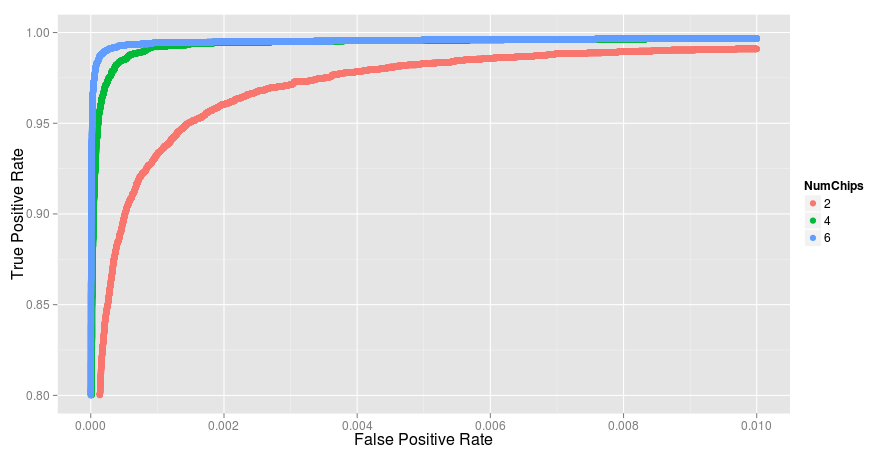
\includegraphics[width=5in]{ecoli-roc.png}\end{center}
\caption{ ROC for $^\textrm{m6}$A detection in \emph{E.coli} genome }
\label{fig:ecoli-roc}
\end{figure}

\subsection{Identification Performance}

We tested the modification identification capability on the bacteria \emph{Desulfurobacterium thermolithotrophum}, which carries RM systems using \mA, \mC{5}, and \mC{4} modifications. The motif CA\textbf{C}C is modified with \mC{4}, GG\textbf{C}C with \mC{5}, and G\textbf{A}TC with \mA. Table \ref{table-confusion} shows that we can accurately separate \mC{4} and \mC{5} modifications, while accurately calling \mA. The TET treatment protocol that amplifies the \mC{5} signal appears to negatively impact the strength of the \mC{4} signal.  Work is in progress to mitigate this effect during the sample preparation.

\begin{table}
\centering
\begin{tabular}{c c c c c c}
Motif & Not Detected & \mC{4} & \mC{5} & \mA & modified\_base \\
\hline 
CACC &   3830 &  \textbf{1222} &    10 &    0  &      114 \\
GGCC &    235 &    0 & \textbf{1065} &    0  &       4  \\
GATC &    66 &    0 &    0 & \textbf{4836}  &       0 \\
None &     &   85 &   98 &   93  &       21799  \\
\end{tabular}
\caption{Modification Identification Confusion Matrix}
\label{table-confusion}
\end{table}


\bibdata{kinetics}
\bibliography{kinetics}
\bibliographystyle{unsrt}

\vspace{1in}

\small{
For Research Use Only. Not for use in diagnostic procedures. © Copyright 2012, Pacific Biosciences of California, Inc. All rights reserved. Information in this document is subject to change without notice. Pacific Biosciences assumes no responsibility for any errors or omissions in this document. Certain notices, terms, conditions and/or use restrictions may pertain to your use of Pacific Biosciences products and/or third party products. Please refer to the applicable Pacific Biosciences Terms and Conditions of Sale and to the applicable license terms at \url{http://www.pacificbiosciences.com/licenses.html}.
Pacific Biosciences, the Pacific Biosciences logo, PacBio, SMRT and SMRTbell are trademarks of Pacific Biosciences in the United States and/or certain other countries. All other trademarks are the sole property of their respective owners.  }



\end{document} 